\section{Interpolation}
Zu gegebenen Punkten $ ( x_{i}, y_{i} ), i=0, ..., n $ mit $ x_{i} \neq x_{j} $ für $ i \neq  j $ eine Funktion G ( dies ist nicht eindeutig! Abhängig von der Funktionsklasse ), so dass $ G ( x_{i} ) = y_{i}, i=0, ..., n $ (Interpolationsbedingung). Interpolation ist \textbf{ungeeignet} für verauschte Daten. Lösung: Approximation der kleinsten Quadrate.
\subsection{Vandermonde/klassisch}
Unterschiedliche Darstellungen für ein Interpolationspolynom $ G(x) = p_{n}(x) $ vom Grad $ n $ haben unterschiedliche Eigenschaften bei der numerischen Berechnung.\textbf{Monombasis:} $ x^{0}, x^{1}, x^{2}, x^{3}, ...; p_{n}(x) = a_{n} x^n + ... + a_{1} x^{1} + a_{0} x^{0} $; 
\textbf{Ziel:} Bestimmung d. Koeffizienten $ a_{0}, a_{1}, ..., a_{n} $ sodass $ p_{n}( x_{i} ) = y_{i} = a_{n} x_{i}^n + ... + a_{1} x_{i}^1 +a_{0} x^{0} $ für i = 0, ..., n; 
\textbf{Für die eindeutige Lösung n+1 Gleichungen: Interpolationsbedingungen};
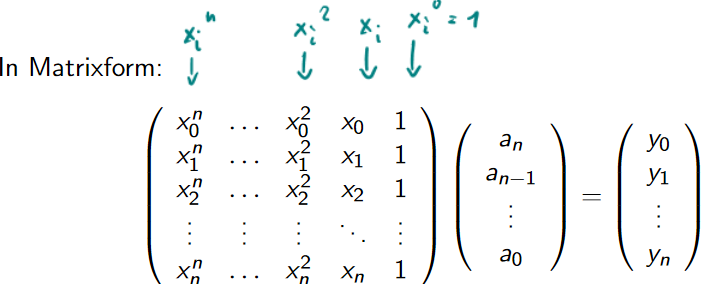
\includegraphics[scale=0.25]{./pic/VandermondeMatrix.png}
Die Koeffizientenmatrix ist die sog. \textbf{Vandermonde Matrix}; \textbf{Eigenschaften:} Die Vandermonde Matrix ist nicht singulär( falls alle $ x_{i} $ verschieden); Rechenaufwand: ${\mathcal O ( n^{3} ) }$; Für große n sehr schlecht konditioniert \& als Allgemeiner Ansatz ungeeignet.
\subsection{Lagrange}